\documentclass[1p]{elsarticle_modified}
%\bibliographystyle{elsarticle-num}

%\usepackage[colorlinks]{hyperref}
%\usepackage{abbrmath_seonhwa} %\Abb, \Ascr, \Acal ,\Abf, \Afrak
\usepackage{amsfonts}
\usepackage{amssymb}
\usepackage{amsmath}
\usepackage{amsthm}
\usepackage{scalefnt}
\usepackage{amsbsy}
\usepackage{kotex}
\usepackage{caption}
\usepackage{subfig}
\usepackage{color}
\usepackage{graphicx}
\usepackage{xcolor} %% white, black, red, green, blue, cyan, magenta, yellow
\usepackage{float}
\usepackage{setspace}
\usepackage{hyperref}

\usepackage{tikz}
\usetikzlibrary{arrows}

\usepackage{multirow}
\usepackage{array} % fixed length table
\usepackage{hhline}

%%%%%%%%%%%%%%%%%%%%%
\makeatletter
\renewcommand*\env@matrix[1][\arraystretch]{%
	\edef\arraystretch{#1}%
	\hskip -\arraycolsep
	\let\@ifnextchar\new@ifnextchar
	\array{*\c@MaxMatrixCols c}}
\makeatother %https://tex.stackexchange.com/questions/14071/how-can-i-increase-the-line-spacing-in-a-matrix
%%%%%%%%%%%%%%%

\usepackage[normalem]{ulem}

\newcommand{\msout}[1]{\ifmmode\text{\sout{\ensuremath{#1}}}\else\sout{#1}\fi}
%SOURCE: \msout is \stkout macro in https://tex.stackexchange.com/questions/20609/strikeout-in-math-mode

\newcommand{\cancel}[1]{
	\ifmmode
	{\color{red}\msout{#1}}
	\else
	{\color{red}\sout{#1}}
	\fi
}

\newcommand{\add}[1]{
	{\color{blue}\uwave{#1}}
}

\newcommand{\replace}[2]{
	\ifmmode
	{\color{red}\msout{#1}}{\color{blue}\uwave{#2}}
	\else
	{\color{red}\sout{#1}}{\color{blue}\uwave{#2}}
	\fi
}

\newcommand{\Sol}{\mathcal{S}} %segment
\newcommand{\D}{D} %diagram
\newcommand{\A}{\mathcal{A}} %arc


%%%%%%%%%%%%%%%%%%%%%%%%%%%%%5 test

\def\sl{\operatorname{\textup{SL}}(2,\Cbb)}
\def\psl{\operatorname{\textup{PSL}}(2,\Cbb)}
\def\quan{\mkern 1mu \triangleright \mkern 1mu}

\theoremstyle{definition}
\newtheorem{thm}{Theorem}[section]
\newtheorem{prop}[thm]{Proposition}
\newtheorem{lem}[thm]{Lemma}
\newtheorem{ques}[thm]{Question}
\newtheorem{cor}[thm]{Corollary}
\newtheorem{defn}[thm]{Definition}
\newtheorem{exam}[thm]{Example}
\newtheorem{rmk}[thm]{Remark}
\newtheorem{alg}[thm]{Algorithm}

\newcommand{\I}{\sqrt{-1}}
\begin{document}

%\begin{frontmatter}
%
%\title{Boundary parabolic representations of knots up to 8 crossings}
%
%%% Group authors per affiliation:
%\author{Yunhi Cho} 
%\address{Department of Mathematics, University of Seoul, Seoul, Korea}
%\ead{yhcho@uos.ac.kr}
%
%
%\author{Seonhwa Kim} %\fnref{s_kim}}
%\address{Center for Geometry and Physics, Institute for Basic Science, Pohang, 37673, Korea}
%\ead{ryeona17@ibs.re.kr}
%
%\author{Hyuk Kim}
%\address{Department of Mathematical Sciences, Seoul National University, Seoul 08826, Korea}
%\ead{hyukkim@snu.ac.kr}
%
%\author{Seokbeom Yoon}
%\address{Department of Mathematical Sciences, Seoul National University, Seoul, 08826,  Korea}
%\ead{sbyoon15@snu.ac.kr}
%
%\begin{abstract}
%We find all boundary parabolic representation of knots up to 8 crossings.
%
%\end{abstract}
%\begin{keyword}
%    \MSC[2010] 57M25 
%\end{keyword}
%
%\end{frontmatter}

%\linenumbers
%\tableofcontents
%
\newcommand\colored[1]{\textcolor{white}{\rule[-0.35ex]{0.8em}{1.4ex}}\kern-0.8em\color{red} #1}%
%\newcommand\colored[1]{\textcolor{white}{ #1}\kern-2.17ex	\textcolor{white}{ #1}\kern-1.81ex	\textcolor{white}{ #1}\kern-2.15ex\color{red}#1	}

{\Large $\underline{12n_{0463}~(K12n_{0463})}$}

\setlength{\tabcolsep}{10pt}
\renewcommand{\arraystretch}{1.6}
\vspace{1cm}\begin{tabular}{m{100pt}>{\centering\arraybackslash}m{274pt}}
\multirow{5}{120pt}{
	\centering
	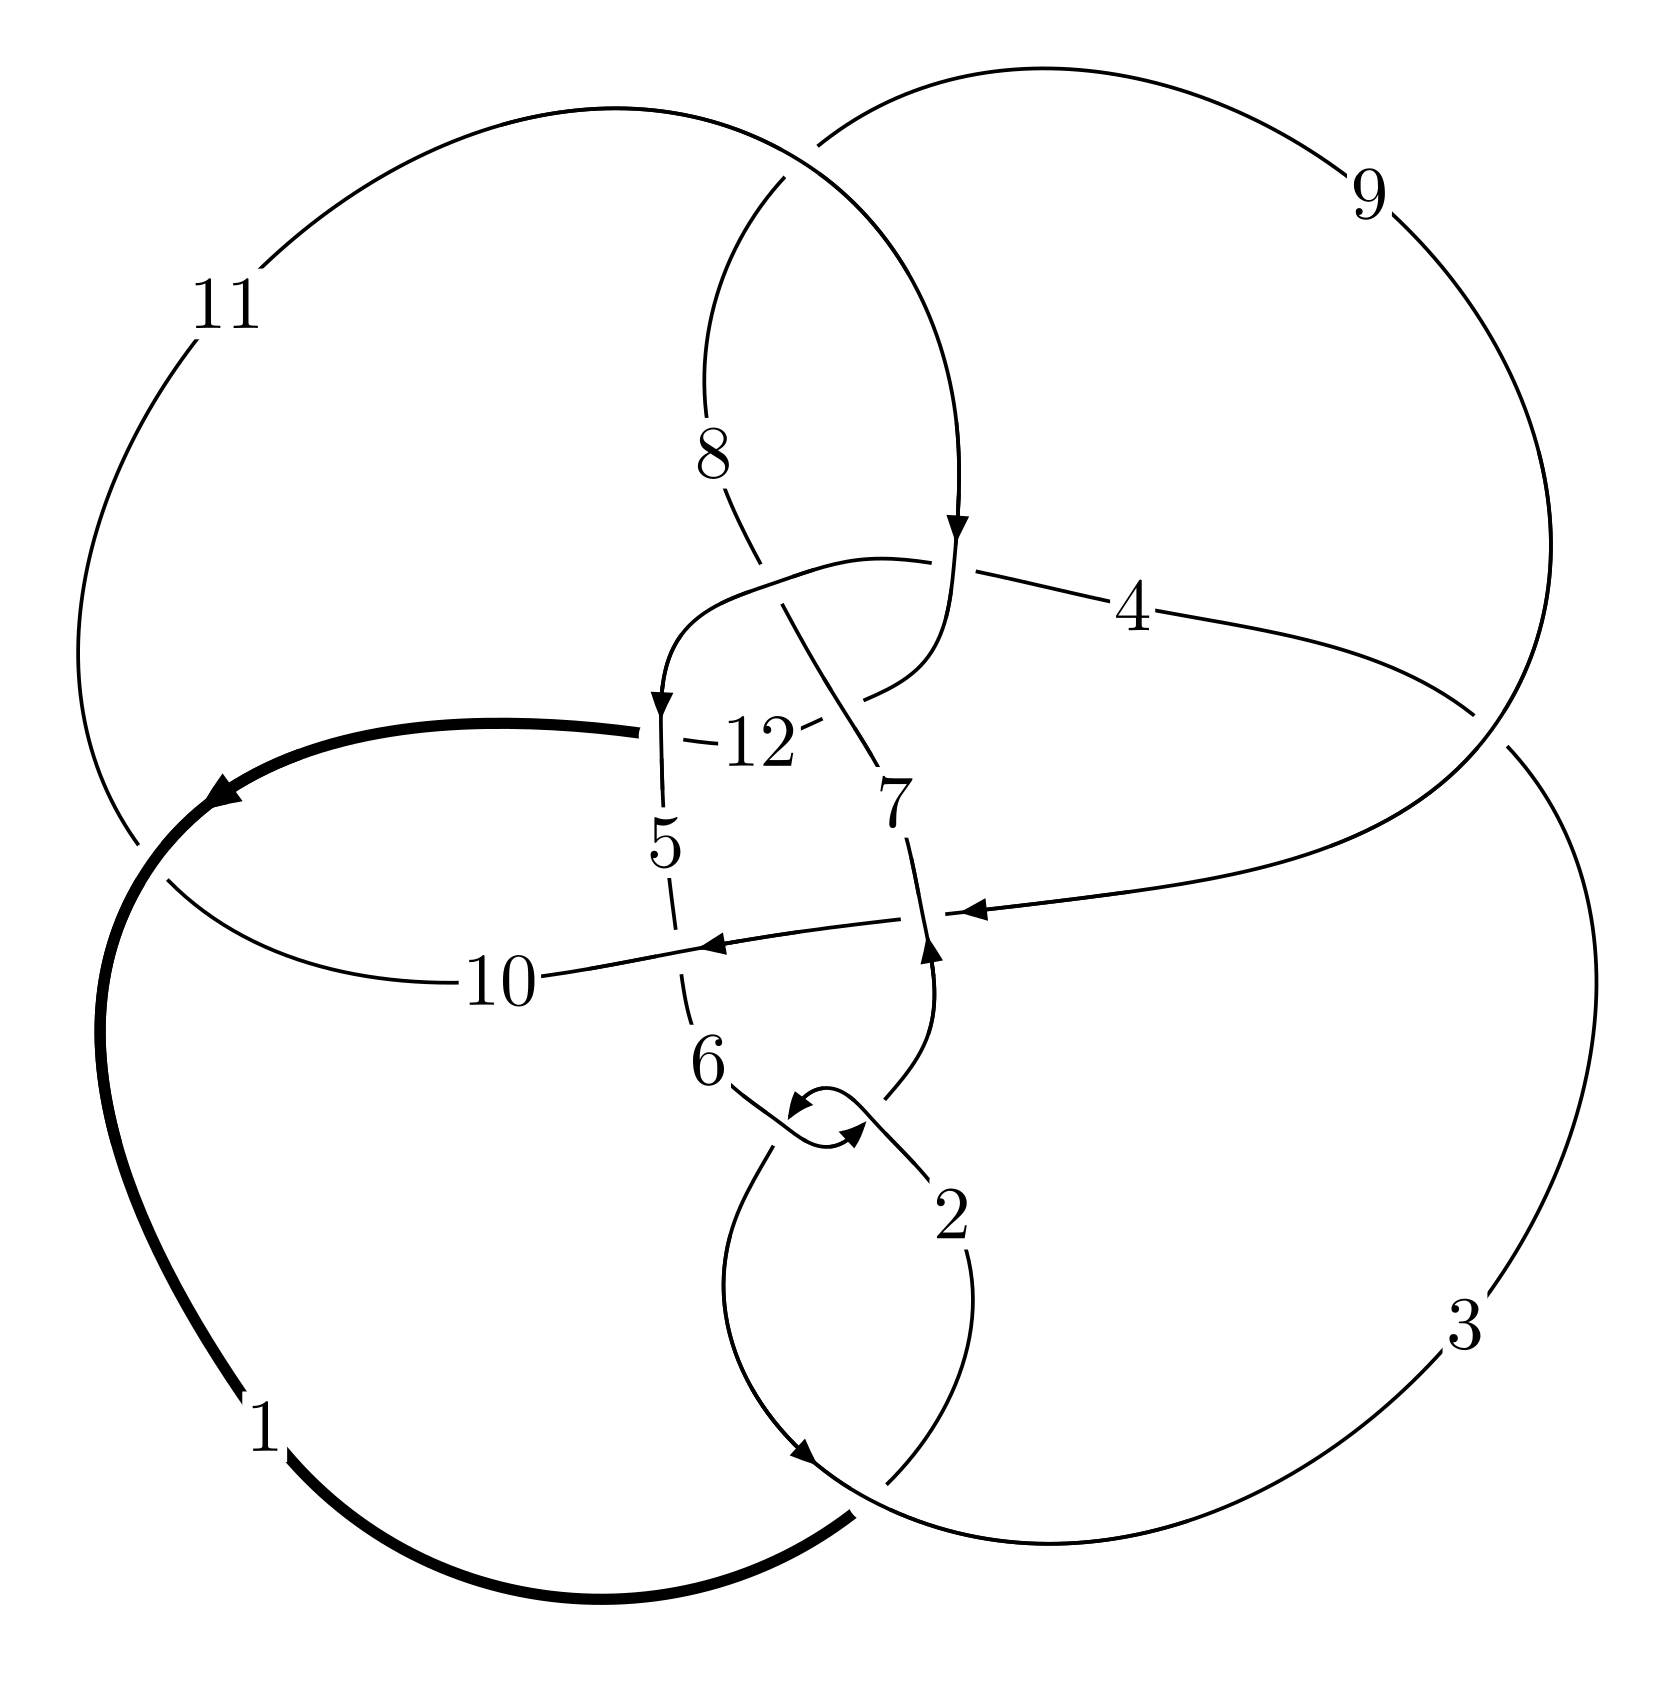
\includegraphics[width=112pt]{../../../GIT/diagram.site/Diagrams/png/2552_12n_0463.png}\\
\ \ \ A knot diagram\footnotemark}&
\allowdisplaybreaks
\textbf{Linearized knot diagam} \\
\cline{2-2}
 &
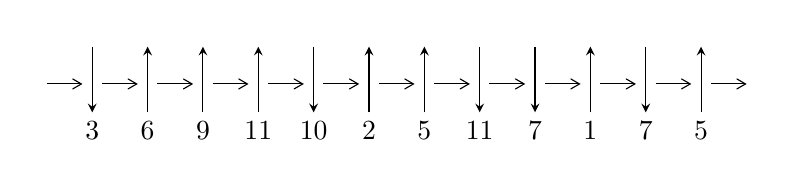
\begin{tikzpicture}[x=20pt, y=17pt]
	% nodes
	\node (C0) at (0, 0) {};
	\node (C1) at (1, 0) {};
	\node (C1U) at (1, +1) {};
	\node (C1D) at (1, -1) {3};

	\node (C2) at (2, 0) {};
	\node (C2U) at (2, +1) {};
	\node (C2D) at (2, -1) {6};

	\node (C3) at (3, 0) {};
	\node (C3U) at (3, +1) {};
	\node (C3D) at (3, -1) {9};

	\node (C4) at (4, 0) {};
	\node (C4U) at (4, +1) {};
	\node (C4D) at (4, -1) {11};

	\node (C5) at (5, 0) {};
	\node (C5U) at (5, +1) {};
	\node (C5D) at (5, -1) {10};

	\node (C6) at (6, 0) {};
	\node (C6U) at (6, +1) {};
	\node (C6D) at (6, -1) {2};

	\node (C7) at (7, 0) {};
	\node (C7U) at (7, +1) {};
	\node (C7D) at (7, -1) {5};

	\node (C8) at (8, 0) {};
	\node (C8U) at (8, +1) {};
	\node (C8D) at (8, -1) {11};

	\node (C9) at (9, 0) {};
	\node (C9U) at (9, +1) {};
	\node (C9D) at (9, -1) {7};

	\node (C10) at (10, 0) {};
	\node (C10U) at (10, +1) {};
	\node (C10D) at (10, -1) {1};

	\node (C11) at (11, 0) {};
	\node (C11U) at (11, +1) {};
	\node (C11D) at (11, -1) {7};

	\node (C12) at (12, 0) {};
	\node (C12U) at (12, +1) {};
	\node (C12D) at (12, -1) {5};
	\node (C13) at (13, 0) {};

	% arrows
	\draw[->,>={angle 60}]
	(C0) edge (C1) (C1) edge (C2) (C2) edge (C3) (C3) edge (C4) (C4) edge (C5) (C5) edge (C6) (C6) edge (C7) (C7) edge (C8) (C8) edge (C9) (C9) edge (C10) (C10) edge (C11) (C11) edge (C12) (C12) edge (C13) ;	\draw[->,>=stealth]
	(C1U) edge (C1D) (C2D) edge (C2U) (C3D) edge (C3U) (C4D) edge (C4U) (C5U) edge (C5D) (C6D) edge (C6U) (C7D) edge (C7U) (C8U) edge (C8D) (C9U) edge (C9D) (C10D) edge (C10U) (C11U) edge (C11D) (C12D) edge (C12U) ;
	\end{tikzpicture} \\
\hhline{~~} \\& 
\textbf{Solving Sequence} \\ \cline{2-2} 
 &
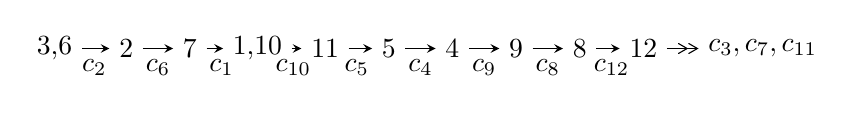
\begin{tikzpicture}[x=23pt, y=7pt]
	% node
	\node (A0) at (-1/8, 0) {3,6};
	\node (A1) at (1, 0) {2};
	\node (A2) at (2, 0) {7};
	\node (A3) at (49/16, 0) {1,10};
	\node (A4) at (33/8, 0) {11};
	\node (A5) at (41/8, 0) {5};
	\node (A6) at (49/8, 0) {4};
	\node (A7) at (57/8, 0) {9};
	\node (A8) at (65/8, 0) {8};
	\node (A9) at (73/8, 0) {12};
	\node (C1) at (1/2, -1) {$c_{2}$};
	\node (C2) at (3/2, -1) {$c_{6}$};
	\node (C3) at (5/2, -1) {$c_{1}$};
	\node (C4) at (29/8, -1) {$c_{10}$};
	\node (C5) at (37/8, -1) {$c_{5}$};
	\node (C6) at (45/8, -1) {$c_{4}$};
	\node (C7) at (53/8, -1) {$c_{9}$};
	\node (C8) at (61/8, -1) {$c_{8}$};
	\node (C9) at (69/8, -1) {$c_{12}$};
	\node (A10) at (11, 0) {$c_{3},c_{7},c_{11}$};

	% edge
	\draw[->,>=stealth]	
	(A0) edge (A1) (A1) edge (A2) (A2) edge (A3) (A3) edge (A4) (A4) edge (A5) (A5) edge (A6) (A6) edge (A7) (A7) edge (A8) (A8) edge (A9) ;
	\draw[->>,>={angle 60}]	
	(A9) edge (A10);
\end{tikzpicture} \\ 

\end{tabular} \\

\footnotetext{
The image of knot diagram is generated by the software ``\textbf{Draw programme}" developed by Andrew Bartholomew(\url{http://www.layer8.co.uk/maths/draw/index.htm\#Running-draw}), where we modified some parts for our purpose(\url{https://github.com/CATsTAILs/LinksPainter}).
}\phantom \\ \newline 
\centering \textbf{Ideals for irreducible components\footnotemark of $X_{\text{par}}$} 
 
\begin{align*}
I^u_{1}&=\langle 
1.95032\times10^{31} u^{56}+1.71447\times10^{31} u^{55}+\cdots+4.19522\times10^{30} b+2.83748\times10^{30},\\
\phantom{I^u_{1}}&\phantom{= \langle  }6.77996\times10^{28} u^{56}+1.77525\times10^{28} u^{55}+\cdots+4.19522\times10^{30} a+2.18312\times10^{31},\;u^{57}+u^{56}+\cdots-4 u+1\rangle \\
I^u_{2}&=\langle 
-22 u^{18}-181 u^{17}+\cdots+163 b-517,\;-236 u^{18}+207 u^{17}+\cdots+489 a-656,\;u^{19}+4 u^{17}+\cdots+u+3\rangle \\
\\
\end{align*}
\raggedright * 2 irreducible components of $\dim_{\mathbb{C}}=0$, with total 76 representations.\\
\footnotetext{All coefficients of polynomials are rational numbers. But the coefficients are sometimes approximated in decimal forms when there is not enough margin.}
\newpage
\renewcommand{\arraystretch}{1}
\centering \section*{I. $I^u_{1}= \langle 1.95\times10^{31} u^{56}+1.71\times10^{31} u^{55}+\cdots+4.20\times10^{30} b+2.84\times10^{30},\;6.78\times10^{28} u^{56}+1.78\times10^{28} u^{55}+\cdots+4.20\times10^{30} a+2.18\times10^{31},\;u^{57}+u^{56}+\cdots-4 u+1 \rangle$}
\flushleft \textbf{(i) Arc colorings}\\
\begin{tabular}{m{7pt} m{180pt} m{7pt} m{180pt} }
\flushright $a_{3}=$&$\begin{pmatrix}1\\0\end{pmatrix}$ \\
\flushright $a_{6}=$&$\begin{pmatrix}0\\u\end{pmatrix}$ \\
\flushright $a_{2}=$&$\begin{pmatrix}1\\u^2\end{pmatrix}$ \\
\flushright $a_{7}=$&$\begin{pmatrix}u\\u^3+u\end{pmatrix}$ \\
\flushright $a_{1}=$&$\begin{pmatrix}u^2+1\\u^2\end{pmatrix}$ \\
\flushright $a_{10}=$&$\begin{pmatrix}-0.0161612 u^{56}-0.00423161 u^{55}+\cdots+9.21492 u-5.20384\\-4.64891 u^{56}-4.08673 u^{55}+\cdots+8.22561 u-0.676360\end{pmatrix}$ \\
\flushright $a_{11}=$&$\begin{pmatrix}1.35701 u^{56}-1.90195 u^{55}+\cdots+15.5812 u-3.61076\\-0.690005 u^{56}-0.579020 u^{55}+\cdots-0.467421 u+2.14333\end{pmatrix}$ \\
\flushright $a_{5}=$&$\begin{pmatrix}0.0705764 u^{56}+1.77602 u^{55}+\cdots+7.98057 u-8.40092\\-1.38197 u^{56}-3.25826 u^{55}+\cdots+15.1658 u-1.78365\end{pmatrix}$ \\
\flushright $a_{4}=$&$\begin{pmatrix}-3.43593 u^{56}-4.84658 u^{55}+\cdots+27.2515 u-12.4708\\0.831823 u^{56}+1.66029 u^{55}+\cdots-4.45631 u+2.03328\end{pmatrix}$ \\
\flushright $a_{9}=$&$\begin{pmatrix}2.85272 u^{56}-0.882312 u^{55}+\cdots+16.7462 u-5.66879\\-1.66635 u^{56}-1.20242 u^{55}+\cdots-2.09986 u+2.60564\end{pmatrix}$ \\
\flushright $a_{8}=$&$\begin{pmatrix}-2.83296 u^{56}-0.179396 u^{55}+\cdots-13.2309 u+6.27694\\-1.18756 u^{56}-1.89146 u^{55}+\cdots+4.35427 u-0.0534336\end{pmatrix}$ \\
\flushright $a_{12}=$&$\begin{pmatrix}-0.245429 u^{56}-0.791586 u^{55}+\cdots+10.2920 u-3.11445\\-2.79987 u^{56}-2.53249 u^{55}+\cdots+6.69697 u-0.0731651\end{pmatrix}$\\&\end{tabular}
\flushleft \textbf{(ii) Obstruction class $= -1$}\\~\\
\flushleft \textbf{(iii) Cusp Shapes $= -1.53377 u^{56}-2.13196 u^{55}+\cdots+30.2938 u-21.3146$}\\~\\
\newpage\renewcommand{\arraystretch}{1}
\flushleft \textbf{(iv) u-Polynomials at the component}\newline \\
\begin{tabular}{m{50pt}|m{274pt}}
Crossings & \hspace{64pt}u-Polynomials at each crossing \\
\hline $$\begin{aligned}c_{1}\end{aligned}$$&$\begin{aligned}
&u^{57}+25 u^{56}+\cdots+14 u-1
\end{aligned}$\\
\hline $$\begin{aligned}c_{2},c_{6}\end{aligned}$$&$\begin{aligned}
&u^{57}- u^{56}+\cdots-4 u-1
\end{aligned}$\\
\hline $$\begin{aligned}c_{3},c_{7}\end{aligned}$$&$\begin{aligned}
&u^{57}+u^{56}+\cdots+20 u-1
\end{aligned}$\\
\hline $$\begin{aligned}c_{4}\end{aligned}$$&$\begin{aligned}
&u^{57}+57 u^{55}+\cdots-5 u-1
\end{aligned}$\\
\hline $$\begin{aligned}c_{5}\end{aligned}$$&$\begin{aligned}
&u^{57}+2 u^{56}+\cdots-20 u-8
\end{aligned}$\\
\hline $$\begin{aligned}c_{8}\end{aligned}$$&$\begin{aligned}
&u^{57}+12 u^{56}+\cdots+6371062 u-656059
\end{aligned}$\\
\hline $$\begin{aligned}c_{9}\end{aligned}$$&$\begin{aligned}
&u^{57}-16 u^{56}+\cdots+4109 u-103
\end{aligned}$\\
\hline $$\begin{aligned}c_{10}\end{aligned}$$&$\begin{aligned}
&u^{57}+17 u^{56}+\cdots-1408 u-121
\end{aligned}$\\
\hline $$\begin{aligned}c_{11}\end{aligned}$$&$\begin{aligned}
&u^{57}-2 u^{56}+\cdots+2391 u-4381
\end{aligned}$\\
\hline $$\begin{aligned}c_{12}\end{aligned}$$&$\begin{aligned}
&u^{57}-5 u^{56}+\cdots-406462 u-931379
\end{aligned}$\\
\hline
\end{tabular}\\~\\
\newpage\renewcommand{\arraystretch}{1}
\flushleft \textbf{(v) Riley Polynomials at the component}\newline \\
\begin{tabular}{m{50pt}|m{274pt}}
Crossings & \hspace{64pt}Riley Polynomials at each crossing \\
\hline $$\begin{aligned}c_{1}\end{aligned}$$&$\begin{aligned}
&y^{57}+17 y^{56}+\cdots+290 y-1
\end{aligned}$\\
\hline $$\begin{aligned}c_{2},c_{6}\end{aligned}$$&$\begin{aligned}
&y^{57}+25 y^{56}+\cdots+14 y-1
\end{aligned}$\\
\hline $$\begin{aligned}c_{3},c_{7}\end{aligned}$$&$\begin{aligned}
&y^{57}+81 y^{56}+\cdots-90 y-1
\end{aligned}$\\
\hline $$\begin{aligned}c_{4}\end{aligned}$$&$\begin{aligned}
&y^{57}+114 y^{56}+\cdots-39 y-1
\end{aligned}$\\
\hline $$\begin{aligned}c_{5}\end{aligned}$$&$\begin{aligned}
&y^{57}-6 y^{56}+\cdots+3024 y-64
\end{aligned}$\\
\hline $$\begin{aligned}c_{8}\end{aligned}$$&$\begin{aligned}
&y^{57}-102 y^{56}+\cdots+13754392721800 y-430413411481
\end{aligned}$\\
\hline $$\begin{aligned}c_{9}\end{aligned}$$&$\begin{aligned}
&y^{57}-40 y^{56}+\cdots+8276171 y-10609
\end{aligned}$\\
\hline $$\begin{aligned}c_{10}\end{aligned}$$&$\begin{aligned}
&y^{57}+5 y^{56}+\cdots-20328 y-14641
\end{aligned}$\\
\hline $$\begin{aligned}c_{11}\end{aligned}$$&$\begin{aligned}
&y^{57}-106 y^{56}+\cdots-199156203 y-19193161
\end{aligned}$\\
\hline $$\begin{aligned}c_{12}\end{aligned}$$&$\begin{aligned}
&y^{57}+47 y^{56}+\cdots-15214664971620 y-867466841641
\end{aligned}$\\
\hline
\end{tabular}\\~\\
\newpage\flushleft \textbf{(vi) Complex Volumes and Cusp Shapes}
$$\begin{array}{c|c|c}  
\text{Solutions to }I^u_{1}& \I (\text{vol} + \sqrt{-1}CS) & \text{Cusp shape}\\
 \hline 
\begin{aligned}
u &= -0.349956 + 0.946672 I \\
a &= -0.303689 - 0.199224 I \\
b &= -2.29980 - 2.68295 I\end{aligned}
 & -12.39530 - 1.32883 I & -10.52705 + 0.14046 I \\ \hline\begin{aligned}
u &= -0.349956 - 0.946672 I \\
a &= -0.303689 + 0.199224 I \\
b &= -2.29980 + 2.68295 I\end{aligned}
 & -12.39530 + 1.32883 I & -10.52705 - 0.14046 I \\ \hline\begin{aligned}
u &= -0.924015 + 0.413182 I \\
a &= \phantom{-}1.43213 - 0.45322 I \\
b &= \phantom{-}0.39289 - 1.40886 I\end{aligned}
 & -10.15880 + 9.30058 I & \phantom{-}0.80484 - 3.88564 I \\ \hline\begin{aligned}
u &= -0.924015 - 0.413182 I \\
a &= \phantom{-}1.43213 + 0.45322 I \\
b &= \phantom{-}0.39289 + 1.40886 I\end{aligned}
 & -10.15880 - 9.30058 I & \phantom{-}0.80484 + 3.88564 I \\ \hline\begin{aligned}
u &= -0.966093 + 0.416915 I \\
a &= -0.349131 + 0.038307 I \\
b &= -0.007320 + 0.449427 I\end{aligned}
 & \phantom{-}1.114500 + 0.475775 I & -1.77277 - 7.35288 I \\ \hline\begin{aligned}
u &= -0.966093 - 0.416915 I \\
a &= -0.349131 - 0.038307 I \\
b &= -0.007320 - 0.449427 I\end{aligned}
 & \phantom{-}1.114500 - 0.475775 I & -1.77277 + 7.35288 I \\ \hline\begin{aligned}
u &= \phantom{-}0.321525 + 1.004170 I \\
a &= -1.47698 - 1.06277 I \\
b &= \phantom{-}1.04811 - 2.34391 I\end{aligned}
 & -13.15110 + 0.96971 I & -6.75666 - 1.21694 I \\ \hline\begin{aligned}
u &= \phantom{-}0.321525 - 1.004170 I \\
a &= -1.47698 + 1.06277 I \\
b &= \phantom{-}1.04811 + 2.34391 I\end{aligned}
 & -13.15110 - 0.96971 I & -6.75666 + 1.21694 I \\ \hline\begin{aligned}
u &= -0.276056 + 0.903211 I \\
a &= -0.236831 - 1.280450 I \\
b &= -0.587986 - 0.401848 I\end{aligned}
 & -1.86758 - 2.05981 I & -0.46331 + 1.96537 I \\ \hline\begin{aligned}
u &= -0.276056 - 0.903211 I \\
a &= -0.236831 + 1.280450 I \\
b &= -0.587986 + 0.401848 I\end{aligned}
 & -1.86758 + 2.05981 I & -0.46331 - 1.96537 I\\
 \hline 
 \end{array}$$\newpage$$\begin{array}{c|c|c}  
\text{Solutions to }I^u_{1}& \I (\text{vol} + \sqrt{-1}CS) & \text{Cusp shape}\\
 \hline 
\begin{aligned}
u &= \phantom{-}0.846735 + 0.415561 I \\
a &= \phantom{-}1.293880 + 0.511117 I \\
b &= \phantom{-}0.365878 + 1.061840 I\end{aligned}
 & \phantom{-}0.02058 - 4.34656 I & \phantom{-}0.26821 + 3.69834 I \\ \hline\begin{aligned}
u &= \phantom{-}0.846735 - 0.415561 I \\
a &= \phantom{-}1.293880 - 0.511117 I \\
b &= \phantom{-}0.365878 - 1.061840 I\end{aligned}
 & \phantom{-}0.02058 + 4.34656 I & \phantom{-}0.26821 - 3.69834 I \\ \hline\begin{aligned}
u &= \phantom{-}0.397636 + 0.979748 I \\
a &= -0.015757 + 0.428561 I \\
b &= -1.39141 + 1.12780 I\end{aligned}
 & -3.43752 + 1.28189 I & -5.91191 - 1.08703 I \\ \hline\begin{aligned}
u &= \phantom{-}0.397636 - 0.979748 I \\
a &= -0.015757 - 0.428561 I \\
b &= -1.39141 - 1.12780 I\end{aligned}
 & -3.43752 - 1.28189 I & -5.91191 + 1.08703 I \\ \hline\begin{aligned}
u &= -0.408296 + 0.978654 I \\
a &= \phantom{-}1.27837 + 0.98027 I \\
b &= \phantom{-}0.910664 - 0.028975 I\end{aligned}
 & -2.61713 - 0.73681 I & -3.54054 + 3.15346 I \\ \hline\begin{aligned}
u &= -0.408296 - 0.978654 I \\
a &= \phantom{-}1.27837 - 0.98027 I \\
b &= \phantom{-}0.910664 + 0.028975 I\end{aligned}
 & -2.61713 + 0.73681 I & -3.54054 - 3.15346 I \\ \hline\begin{aligned}
u &= -0.675685 + 0.597241 I \\
a &= \phantom{-}0.876923 - 0.578864 I \\
b &= -0.097247 - 0.847074 I\end{aligned}
 & \phantom{-}1.50545 - 1.28490 I & \phantom{-}3.77323 + 4.50863 I \\ \hline\begin{aligned}
u &= -0.675685 - 0.597241 I \\
a &= \phantom{-}0.876923 + 0.578864 I \\
b &= -0.097247 + 0.847074 I\end{aligned}
 & \phantom{-}1.50545 + 1.28490 I & \phantom{-}3.77323 - 4.50863 I \\ \hline\begin{aligned}
u &= \phantom{-}0.459215 + 1.005020 I \\
a &= -0.284902 + 0.841083 I \\
b &= \phantom{-}0.106017 + 1.132020 I\end{aligned}
 & -3.04982 + 4.72917 I & -4.15324 - 9.32450 I \\ \hline\begin{aligned}
u &= \phantom{-}0.459215 - 1.005020 I \\
a &= -0.284902 - 0.841083 I \\
b &= \phantom{-}0.106017 - 1.132020 I\end{aligned}
 & -3.04982 - 4.72917 I & -4.15324 + 9.32450 I\\
 \hline 
 \end{array}$$\newpage$$\begin{array}{c|c|c}  
\text{Solutions to }I^u_{1}& \I (\text{vol} + \sqrt{-1}CS) & \text{Cusp shape}\\
 \hline 
\begin{aligned}
u &= \phantom{-}0.711622 + 0.542227 I \\
a &= -0.978562 - 0.301016 I \\
b &= \phantom{-}0.115817 - 1.372610 I\end{aligned}
 & \phantom{-}2.68108 - 2.12211 I & \phantom{-}6.33969 + 1.94365 I \\ \hline\begin{aligned}
u &= \phantom{-}0.711622 - 0.542227 I \\
a &= -0.978562 + 0.301016 I \\
b &= \phantom{-}0.115817 + 1.372610 I\end{aligned}
 & \phantom{-}2.68108 + 2.12211 I & \phantom{-}6.33969 - 1.94365 I \\ \hline\begin{aligned}
u &= -0.501529 + 1.005740 I \\
a &= -0.67417 + 1.37103 I \\
b &= \phantom{-}1.67778 + 2.16523 I\end{aligned}
 & -1.95552 - 5.12176 I & \phantom{-0.000000 -}0. + 6.61060 I \\ \hline\begin{aligned}
u &= -0.501529 - 1.005740 I \\
a &= -0.67417 - 1.37103 I \\
b &= \phantom{-}1.67778 - 2.16523 I\end{aligned}
 & -1.95552 + 5.12176 I & \phantom{-0.000000 } 0. - 6.61060 I \\ \hline\begin{aligned}
u &= \phantom{-}0.199034 + 0.817620 I \\
a &= \phantom{-}0.803863 - 0.976801 I \\
b &= -0.276848 - 0.608793 I\end{aligned}
 & -1.70481 - 1.56112 I & -0.16745 + 5.41560 I \\ \hline\begin{aligned}
u &= \phantom{-}0.199034 - 0.817620 I \\
a &= \phantom{-}0.803863 + 0.976801 I \\
b &= -0.276848 + 0.608793 I\end{aligned}
 & -1.70481 + 1.56112 I & -0.16745 - 5.41560 I \\ \hline\begin{aligned}
u &= -0.538375 + 1.030800 I \\
a &= -0.116672 - 0.787747 I \\
b &= \phantom{-}0.28486 - 2.44669 I\end{aligned}
 & -10.96040 - 4.57401 I & \phantom{-0.000000 } 0 \\ \hline\begin{aligned}
u &= -0.538375 - 1.030800 I \\
a &= -0.116672 + 0.787747 I \\
b &= \phantom{-}0.28486 + 2.44669 I\end{aligned}
 & -10.96040 + 4.57401 I & \phantom{-0.000000 } 0 \\ \hline\begin{aligned}
u &= -0.584272 + 1.019390 I \\
a &= \phantom{-}0.400981 - 0.948656 I \\
b &= -0.83486 - 1.37560 I\end{aligned}
 & \phantom{-}0.20940 - 3.59994 I & \phantom{-0.000000 } 0 \\ \hline\begin{aligned}
u &= -0.584272 - 1.019390 I \\
a &= \phantom{-}0.400981 + 0.948656 I \\
b &= -0.83486 + 1.37560 I\end{aligned}
 & \phantom{-}0.20940 + 3.59994 I & \phantom{-0.000000 } 0\\
 \hline 
 \end{array}$$\newpage$$\begin{array}{c|c|c}  
\text{Solutions to }I^u_{1}& \I (\text{vol} + \sqrt{-1}CS) & \text{Cusp shape}\\
 \hline 
\begin{aligned}
u &= \phantom{-}0.527359 + 1.065210 I \\
a &= \phantom{-}1.64010 - 0.51000 I \\
b &= \phantom{-}0.93686 + 1.21045 I\end{aligned}
 & -11.70070 + 5.59902 I & \phantom{-0.000000 } 0 \\ \hline\begin{aligned}
u &= \phantom{-}0.527359 - 1.065210 I \\
a &= \phantom{-}1.64010 + 0.51000 I \\
b &= \phantom{-}0.93686 - 1.21045 I\end{aligned}
 & -11.70070 - 5.59902 I & \phantom{-0.000000 } 0 \\ \hline\begin{aligned}
u &= \phantom{-}0.996785 + 0.661596 I \\
a &= -0.195695 + 0.706856 I \\
b &= -0.836567 + 0.341424 I\end{aligned}
 & -8.63281 + 4.27743 I & \phantom{-0.000000 } 0 \\ \hline\begin{aligned}
u &= \phantom{-}0.996785 - 0.661596 I \\
a &= -0.195695 - 0.706856 I \\
b &= -0.836567 - 0.341424 I\end{aligned}
 & -8.63281 - 4.27743 I & \phantom{-0.000000 } 0 \\ \hline\begin{aligned}
u &= \phantom{-}0.605290 + 1.038470 I \\
a &= -0.327621 - 0.864561 I \\
b &= \phantom{-}1.42976 - 1.72470 I\end{aligned}
 & \phantom{-}1.19878 + 7.18626 I & \phantom{-0.000000 } 0 \\ \hline\begin{aligned}
u &= \phantom{-}0.605290 - 1.038470 I \\
a &= -0.327621 + 0.864561 I \\
b &= \phantom{-}1.42976 + 1.72470 I\end{aligned}
 & \phantom{-}1.19878 - 7.18626 I & \phantom{-0.000000 } 0 \\ \hline\begin{aligned}
u &= \phantom{-}0.058017 + 1.216930 I \\
a &= -0.305650 + 0.796434 I \\
b &= -0.521846 + 0.385158 I\end{aligned}
 & -5.73579 - 1.82350 I & \phantom{-0.000000 } 0 \\ \hline\begin{aligned}
u &= \phantom{-}0.058017 - 1.216930 I \\
a &= -0.305650 - 0.796434 I \\
b &= -0.521846 - 0.385158 I\end{aligned}
 & -5.73579 + 1.82350 I & \phantom{-0.000000 } 0 \\ \hline\begin{aligned}
u &= -0.570883 + 0.483592 I \\
a &= \phantom{-}1.42182 + 0.20086 I \\
b &= -1.056060 + 0.012511 I\end{aligned}
 & -9.37580 + 0.10389 I & -0.28028 - 1.50449 I \\ \hline\begin{aligned}
u &= -0.570883 - 0.483592 I \\
a &= \phantom{-}1.42182 - 0.20086 I \\
b &= -1.056060 - 0.012511 I\end{aligned}
 & -9.37580 - 0.10389 I & -0.28028 + 1.50449 I\\
 \hline 
 \end{array}$$\newpage$$\begin{array}{c|c|c}  
\text{Solutions to }I^u_{1}& \I (\text{vol} + \sqrt{-1}CS) & \text{Cusp shape}\\
 \hline 
\begin{aligned}
u &= -0.421818 + 0.600652 I \\
a &= -1.77014 + 0.12826 I \\
b &= \phantom{-}0.01207 + 1.76563 I\end{aligned}
 & -0.649695 + 1.123590 I & \phantom{-}1.75264 - 1.62857 I \\ \hline\begin{aligned}
u &= -0.421818 - 0.600652 I \\
a &= -1.77014 - 0.12826 I \\
b &= \phantom{-}0.01207 - 1.76563 I\end{aligned}
 & -0.649695 - 1.123590 I & \phantom{-}1.75264 + 1.62857 I \\ \hline\begin{aligned}
u &= \phantom{-}0.625228 + 1.120040 I \\
a &= \phantom{-}0.285068 + 1.206890 I \\
b &= -1.23895 + 1.72070 I\end{aligned}
 & -2.08741 + 9.80069 I & \phantom{-0.000000 } 0 \\ \hline\begin{aligned}
u &= \phantom{-}0.625228 - 1.120040 I \\
a &= \phantom{-}0.285068 - 1.206890 I \\
b &= -1.23895 - 1.72070 I\end{aligned}
 & -2.08741 - 9.80069 I & \phantom{-0.000000 } 0 \\ \hline\begin{aligned}
u &= -0.075556 + 1.291700 I \\
a &= -0.595125 - 0.881595 I \\
b &= -0.251519 - 0.446971 I\end{aligned}
 & -16.3180 + 6.3103 I & \phantom{-0.000000 } 0 \\ \hline\begin{aligned}
u &= -0.075556 - 1.291700 I \\
a &= -0.595125 + 0.881595 I \\
b &= -0.251519 + 0.446971 I\end{aligned}
 & -16.3180 - 6.3103 I & \phantom{-0.000000 } 0 \\ \hline\begin{aligned}
u &= \phantom{-}0.595217 + 0.376896 I \\
a &= -0.49225 + 2.24517 I \\
b &= -0.95401 + 1.43916 I\end{aligned}
 & -9.74503 - 1.13283 I & \phantom{-}0.125687 + 0.944361 I \\ \hline\begin{aligned}
u &= \phantom{-}0.595217 - 0.376896 I \\
a &= -0.49225 - 2.24517 I \\
b &= -0.95401 - 1.43916 I\end{aligned}
 & -9.74503 + 1.13283 I & \phantom{-}0.125687 - 0.944361 I \\ \hline\begin{aligned}
u &= -0.652334 + 1.131340 I \\
a &= -0.054821 + 0.544694 I \\
b &= \phantom{-}0.97755 + 1.04049 I\end{aligned}
 & -1.05681 - 6.25223 I & \phantom{-0.000000 } 0 \\ \hline\begin{aligned}
u &= -0.652334 - 1.131340 I \\
a &= -0.054821 - 0.544694 I \\
b &= \phantom{-}0.97755 - 1.04049 I\end{aligned}
 & -1.05681 + 6.25223 I & \phantom{-0.000000 } 0\\
 \hline 
 \end{array}$$\newpage$$\begin{array}{c|c|c}  
\text{Solutions to }I^u_{1}& \I (\text{vol} + \sqrt{-1}CS) & \text{Cusp shape}\\
 \hline 
\begin{aligned}
u &= -0.648644 + 1.154300 I \\
a &= \phantom{-}0.242666 - 1.233560 I \\
b &= -1.57143 - 2.00829 I\end{aligned}
 & -12.4207 - 15.0539 I & \phantom{-0.000000 } 0 \\ \hline\begin{aligned}
u &= -0.648644 - 1.154300 I \\
a &= \phantom{-}0.242666 + 1.233560 I \\
b &= -1.57143 + 2.00829 I\end{aligned}
 & -12.4207 + 15.0539 I & \phantom{-0.000000 } 0 \\ \hline\begin{aligned}
u &= -0.671768\phantom{ +0.000000I} \\
a &= \phantom{-}0.366130\phantom{ +0.000000I} \\
b &= \phantom{-}0.477596\phantom{ +0.000000I}\end{aligned}
 & \phantom{-}1.20012\phantom{ +0.000000I} & \phantom{-}11.5930\phantom{ +0.000000I} \\ \hline\begin{aligned}
u &= \phantom{-}0.80509 + 1.19177 I \\
a &= \phantom{-}0.354067 - 0.302190 I \\
b &= \phantom{-}0.803093 + 0.109041 I\end{aligned}
 & -10.20330 + 2.47505 I & \phantom{-0.000000 } 0 \\ \hline\begin{aligned}
u &= \phantom{-}0.80509 - 1.19177 I \\
a &= \phantom{-}0.354067 + 0.302190 I \\
b &= \phantom{-}0.803093 - 0.109041 I\end{aligned}
 & -10.20330 - 2.47505 I & \phantom{-0.000000 } 0 \\ \hline\begin{aligned}
u &= \phantom{-}0.280643 + 0.019804 I \\
a &= \phantom{-}2.46507 + 1.48163 I \\
b &= \phantom{-}0.125719 - 0.515240 I\end{aligned}
 & -1.21526 - 1.45435 I & -0.50304 + 4.00620 I \\ \hline\begin{aligned}
u &= \phantom{-}0.280643 - 0.019804 I \\
a &= \phantom{-}2.46507 - 1.48163 I \\
b &= \phantom{-}0.125719 + 0.515240 I\end{aligned}
 & -1.21526 + 1.45435 I & -0.50304 - 4.00620 I\\
 \hline 
 \end{array}$$\newpage\newpage\renewcommand{\arraystretch}{1}
\centering \section*{II. $I^u_{2}= \langle -22 u^{18}-181 u^{17}+\cdots+163 b-517,\;-236 u^{18}+207 u^{17}+\cdots+489 a-656,\;u^{19}+4 u^{17}+\cdots+u+3 \rangle$}
\flushleft \textbf{(i) Arc colorings}\\
\begin{tabular}{m{7pt} m{180pt} m{7pt} m{180pt} }
\flushright $a_{3}=$&$\begin{pmatrix}1\\0\end{pmatrix}$ \\
\flushright $a_{6}=$&$\begin{pmatrix}0\\u\end{pmatrix}$ \\
\flushright $a_{2}=$&$\begin{pmatrix}1\\u^2\end{pmatrix}$ \\
\flushright $a_{7}=$&$\begin{pmatrix}u\\u^3+u\end{pmatrix}$ \\
\flushright $a_{1}=$&$\begin{pmatrix}u^2+1\\u^2\end{pmatrix}$ \\
\flushright $a_{10}=$&$\begin{pmatrix}0.482618 u^{18}-0.423313 u^{17}+\cdots+2.27198 u+1.34151\\0.134969 u^{18}+1.11043 u^{17}+\cdots+2.71166 u+3.17178\end{pmatrix}$ \\
\flushright $a_{11}=$&$\begin{pmatrix}1.01022 u^{18}-0.809816 u^{17}+\cdots+2.78119 u+0.740286\\u^{17}+4 u^{15}+\cdots+u+4\end{pmatrix}$ \\
\flushright $a_{5}=$&$\begin{pmatrix}-0.750511 u^{18}-0.159509 u^{17}+\cdots-0.139059 u-2.13701\\1.43558 u^{18}-0.0981595 u^{17}+\cdots+4.47853 u-1.26380\end{pmatrix}$ \\
\flushright $a_{4}=$&$\begin{pmatrix}0.523517 u^{18}+0.337423 u^{17}+\cdots+2.39673 u-1.69734\\-0.533742 u^{18}-0.527607 u^{17}+\cdots-1.17791 u-0.0429448\end{pmatrix}$ \\
\flushright $a_{9}=$&$\begin{pmatrix}1.43967 u^{18}-0.822086 u^{17}+\cdots+2.59100 u-0.167689\\-0.325153 u^{18}+0.552147 u^{17}+\cdots+0.558282 u+2.85890\end{pmatrix}$ \\
\flushright $a_{8}=$&$\begin{pmatrix}0.482618 u^{18}-0.423313 u^{17}+\cdots+2.27198 u-2.65849\\0.423313 u^{18}-0.926380 u^{17}+\cdots-1.85890 u-2.55215\end{pmatrix}$ \\
\flushright $a_{12}=$&$\begin{pmatrix}0.482618 u^{18}-0.423313 u^{17}+\cdots+2.27198 u+2.34151\\0.0613497 u^{18}+1.14110 u^{17}+\cdots+1.68712 u+4.44172\end{pmatrix}$\\&\end{tabular}
\flushleft \textbf{(ii) Obstruction class $= 1$}\\~\\
\flushleft \textbf{(iii) Cusp Shapes $= -\frac{52}{163} u^{18}-\frac{87}{163} u^{17}+\cdots-\frac{941}{163} u-\frac{1059}{163}$}\\~\\
\newpage\renewcommand{\arraystretch}{1}
\flushleft \textbf{(iv) u-Polynomials at the component}\newline \\
\begin{tabular}{m{50pt}|m{274pt}}
Crossings & \hspace{64pt}u-Polynomials at each crossing \\
\hline $$\begin{aligned}c_{1}\end{aligned}$$&$\begin{aligned}
&u^{19}-8 u^{18}+\cdots-47 u+9
\end{aligned}$\\
\hline $$\begin{aligned}c_{2}\end{aligned}$$&$\begin{aligned}
&u^{19}+4 u^{17}+\cdots+u+3
\end{aligned}$\\
\hline $$\begin{aligned}c_{3}\end{aligned}$$&$\begin{aligned}
&u^{19}+10 u^{17}+\cdots+3 u+1
\end{aligned}$\\
\hline $$\begin{aligned}c_{4}\end{aligned}$$&$\begin{aligned}
&u^{19}+u^{18}+\cdots+2 u-1
\end{aligned}$\\
\hline $$\begin{aligned}c_{5}\end{aligned}$$&$\begin{aligned}
&u^{19}+u^{18}+\cdots+2 u-1
\end{aligned}$\\
\hline $$\begin{aligned}c_{6}\end{aligned}$$&$\begin{aligned}
&u^{19}+4 u^{17}+\cdots+u-3
\end{aligned}$\\
\hline $$\begin{aligned}c_{7}\end{aligned}$$&$\begin{aligned}
&u^{19}+10 u^{17}+\cdots+3 u-1
\end{aligned}$\\
\hline $$\begin{aligned}c_{8}\end{aligned}$$&$\begin{aligned}
&u^{19}-15 u^{18}+\cdots+17 u-3
\end{aligned}$\\
\hline $$\begin{aligned}c_{9}\end{aligned}$$&$\begin{aligned}
&u^{19}+3 u^{18}+\cdots- u^2+1
\end{aligned}$\\
\hline $$\begin{aligned}c_{10}\end{aligned}$$&$\begin{aligned}
&u^{19}+4 u^{18}+\cdots+5 u+1
\end{aligned}$\\
\hline $$\begin{aligned}c_{11}\end{aligned}$$&$\begin{aligned}
&u^{19}- u^{18}+\cdots+6 u+1
\end{aligned}$\\
\hline $$\begin{aligned}c_{12}\end{aligned}$$&$\begin{aligned}
&u^{19}+2 u^{18}+\cdots- u+1
\end{aligned}$\\
\hline
\end{tabular}\\~\\
\newpage\renewcommand{\arraystretch}{1}
\flushleft \textbf{(v) Riley Polynomials at the component}\newline \\
\begin{tabular}{m{50pt}|m{274pt}}
Crossings & \hspace{64pt}Riley Polynomials at each crossing \\
\hline $$\begin{aligned}c_{1}\end{aligned}$$&$\begin{aligned}
&y^{19}+8 y^{18}+\cdots-131 y-81
\end{aligned}$\\
\hline $$\begin{aligned}c_{2},c_{6}\end{aligned}$$&$\begin{aligned}
&y^{19}+8 y^{18}+\cdots-47 y-9
\end{aligned}$\\
\hline $$\begin{aligned}c_{3},c_{7}\end{aligned}$$&$\begin{aligned}
&y^{19}+20 y^{18}+\cdots-7 y-1
\end{aligned}$\\
\hline $$\begin{aligned}c_{4}\end{aligned}$$&$\begin{aligned}
&y^{19}+13 y^{18}+\cdots+12 y-1
\end{aligned}$\\
\hline $$\begin{aligned}c_{5}\end{aligned}$$&$\begin{aligned}
&y^{19}+y^{18}+\cdots-6 y-1
\end{aligned}$\\
\hline $$\begin{aligned}c_{8}\end{aligned}$$&$\begin{aligned}
&y^{19}-19 y^{18}+\cdots-101 y-9
\end{aligned}$\\
\hline $$\begin{aligned}c_{9}\end{aligned}$$&$\begin{aligned}
&y^{19}-21 y^{18}+\cdots+2 y-1
\end{aligned}$\\
\hline $$\begin{aligned}c_{10}\end{aligned}$$&$\begin{aligned}
&y^{19}-8 y^{18}+\cdots+7 y-1
\end{aligned}$\\
\hline $$\begin{aligned}c_{11}\end{aligned}$$&$\begin{aligned}
&y^{19}-19 y^{18}+\cdots-48 y-1
\end{aligned}$\\
\hline $$\begin{aligned}c_{12}\end{aligned}$$&$\begin{aligned}
&y^{19}+6 y^{18}+\cdots- y-1
\end{aligned}$\\
\hline
\end{tabular}\\~\\
\newpage\flushleft \textbf{(vi) Complex Volumes and Cusp Shapes}
$$\begin{array}{c|c|c}  
\text{Solutions to }I^u_{2}& \I (\text{vol} + \sqrt{-1}CS) & \text{Cusp shape}\\
 \hline 
\begin{aligned}
u &= -0.809380 + 0.609336 I \\
a &= -0.642590 + 0.567390 I \\
b &= -0.033190 + 1.100160 I\end{aligned}
 & \phantom{-}1.93114 + 0.05703 I & \phantom{-}5.27608 - 0.61329 I \\ \hline\begin{aligned}
u &= -0.809380 - 0.609336 I \\
a &= -0.642590 - 0.567390 I \\
b &= -0.033190 - 1.100160 I\end{aligned}
 & \phantom{-}1.93114 - 0.05703 I & \phantom{-}5.27608 + 0.61329 I \\ \hline\begin{aligned}
u &= \phantom{-}0.380702 + 0.892229 I \\
a &= \phantom{-}0.864989 + 0.488196 I \\
b &= -1.45142 + 3.06408 I\end{aligned}
 & -11.73130 + 1.58594 I & \phantom{-}1.69710 - 4.85525 I \\ \hline\begin{aligned}
u &= \phantom{-}0.380702 - 0.892229 I \\
a &= \phantom{-}0.864989 - 0.488196 I \\
b &= -1.45142 - 3.06408 I\end{aligned}
 & -11.73130 - 1.58594 I & \phantom{-}1.69710 + 4.85525 I \\ \hline\begin{aligned}
u &= -0.950794\phantom{ +0.000000I} \\
a &= \phantom{-}0.534200\phantom{ +0.000000I} \\
b &= \phantom{-}0.417548\phantom{ +0.000000I}\end{aligned}
 & \phantom{-}0.736407\phantom{ +0.000000I} & -10.1920\phantom{ +0.000000I} \\ \hline\begin{aligned}
u &= \phantom{-}0.106744 + 1.047650 I \\
a &= \phantom{-}0.605523 - 0.806007 I \\
b &= \phantom{-}0.379570 - 0.884630 I\end{aligned}
 & -3.40808 - 2.06211 I & -4.23882 + 3.25949 I \\ \hline\begin{aligned}
u &= \phantom{-}0.106744 - 1.047650 I \\
a &= \phantom{-}0.605523 + 0.806007 I \\
b &= \phantom{-}0.379570 + 0.884630 I\end{aligned}
 & -3.40808 + 2.06211 I & -4.23882 - 3.25949 I \\ \hline\begin{aligned}
u &= \phantom{-}0.792456 + 0.478311 I \\
a &= -1.237570 - 0.352759 I \\
b &= \phantom{-}0.061164 - 1.114880 I\end{aligned}
 & \phantom{-}1.79413 - 3.68410 I & \phantom{-}3.77498 + 3.60536 I \\ \hline\begin{aligned}
u &= \phantom{-}0.792456 - 0.478311 I \\
a &= -1.237570 + 0.352759 I \\
b &= \phantom{-}0.061164 + 1.114880 I\end{aligned}
 & \phantom{-}1.79413 + 3.68410 I & \phantom{-}3.77498 - 3.60536 I \\ \hline\begin{aligned}
u &= -0.312010 + 0.855320 I \\
a &= \phantom{-}1.26370 + 0.74522 I \\
b &= -0.083954 - 0.552115 I\end{aligned}
 & -1.95432 + 0.51994 I & -3.03581 + 0.54030 I\\
 \hline 
 \end{array}$$\newpage$$\begin{array}{c|c|c}  
\text{Solutions to }I^u_{2}& \I (\text{vol} + \sqrt{-1}CS) & \text{Cusp shape}\\
 \hline 
\begin{aligned}
u &= -0.312010 - 0.855320 I \\
a &= \phantom{-}1.26370 - 0.74522 I \\
b &= -0.083954 + 0.552115 I\end{aligned}
 & -1.95432 - 0.51994 I & -3.03581 - 0.54030 I \\ \hline\begin{aligned}
u &= -0.402259 + 1.014470 I \\
a &= -0.054502 - 1.190310 I \\
b &= -0.90125 - 1.24715 I\end{aligned}
 & -2.70781 - 3.32351 I & -4.18487 + 4.02916 I \\ \hline\begin{aligned}
u &= -0.402259 - 1.014470 I \\
a &= -0.054502 + 1.190310 I \\
b &= -0.90125 + 1.24715 I\end{aligned}
 & -2.70781 + 3.32351 I & -4.18487 - 4.02916 I \\ \hline\begin{aligned}
u &= -0.635239 + 1.022560 I \\
a &= -0.614017 + 0.776240 I \\
b &= \phantom{-}0.90356 + 1.37817 I\end{aligned}
 & \phantom{-}0.65149 - 5.44524 I & \phantom{-}1.78951 + 4.96299 I \\ \hline\begin{aligned}
u &= -0.635239 - 1.022560 I \\
a &= -0.614017 - 0.776240 I \\
b &= \phantom{-}0.90356 - 1.37817 I\end{aligned}
 & \phantom{-}0.65149 + 5.44524 I & \phantom{-}1.78951 - 4.96299 I \\ \hline\begin{aligned}
u &= \phantom{-}0.732861 + 0.997527 I \\
a &= -0.376611 - 0.095684 I \\
b &= -0.241631 + 0.261608 I\end{aligned}
 & -9.58271 + 2.96759 I & -0.28434 - 4.02482 I \\ \hline\begin{aligned}
u &= \phantom{-}0.732861 - 0.997527 I \\
a &= -0.376611 + 0.095684 I \\
b &= -0.241631 - 0.261608 I\end{aligned}
 & -9.58271 - 2.96759 I & -0.28434 + 4.02482 I \\ \hline\begin{aligned}
u &= \phantom{-}0.621521 + 1.087370 I \\
a &= -0.242691 - 1.035660 I \\
b &= \phantom{-}1.15837 - 1.98145 I\end{aligned}
 & -0.03477 + 9.00564 I & \phantom{-}0.80205 - 7.81650 I \\ \hline\begin{aligned}
u &= \phantom{-}0.621521 - 1.087370 I \\
a &= -0.242691 + 1.035660 I \\
b &= \phantom{-}1.15837 + 1.98145 I\end{aligned}
 & -0.03477 - 9.00564 I & \phantom{-}0.80205 + 7.81650 I\\
 \hline 
 \end{array}$$\newpage
\newpage\renewcommand{\arraystretch}{1}
\centering \section*{ III. u-Polynomials}
\begin{tabular}{m{50pt}|m{274pt}}
Crossings & \hspace{64pt}u-Polynomials at each crossing \\
\hline $$\begin{aligned}c_{1}\end{aligned}$$&$\begin{aligned}
&(u^{19}-8 u^{18}+\cdots-47 u+9)(u^{57}+25 u^{56}+\cdots+14 u-1)
\end{aligned}$\\
\hline $$\begin{aligned}c_{2}\end{aligned}$$&$\begin{aligned}
&(u^{19}+4 u^{17}+\cdots+u+3)(u^{57}- u^{56}+\cdots-4 u-1)
\end{aligned}$\\
\hline $$\begin{aligned}c_{3}\end{aligned}$$&$\begin{aligned}
&(u^{19}+10 u^{17}+\cdots+3 u+1)(u^{57}+u^{56}+\cdots+20 u-1)
\end{aligned}$\\
\hline $$\begin{aligned}c_{4}\end{aligned}$$&$\begin{aligned}
&(u^{19}+u^{18}+\cdots+2 u-1)(u^{57}+57 u^{55}+\cdots-5 u-1)
\end{aligned}$\\
\hline $$\begin{aligned}c_{5}\end{aligned}$$&$\begin{aligned}
&(u^{19}+u^{18}+\cdots+2 u-1)(u^{57}+2 u^{56}+\cdots-20 u-8)
\end{aligned}$\\
\hline $$\begin{aligned}c_{6}\end{aligned}$$&$\begin{aligned}
&(u^{19}+4 u^{17}+\cdots+u-3)(u^{57}- u^{56}+\cdots-4 u-1)
\end{aligned}$\\
\hline $$\begin{aligned}c_{7}\end{aligned}$$&$\begin{aligned}
&(u^{19}+10 u^{17}+\cdots+3 u-1)(u^{57}+u^{56}+\cdots+20 u-1)
\end{aligned}$\\
\hline $$\begin{aligned}c_{8}\end{aligned}$$&$\begin{aligned}
&(u^{19}-15 u^{18}+\cdots+17 u-3)\\
&\cdot(u^{57}+12 u^{56}+\cdots+6371062 u-656059)
\end{aligned}$\\
\hline $$\begin{aligned}c_{9}\end{aligned}$$&$\begin{aligned}
&(u^{19}+3 u^{18}+\cdots- u^2+1)(u^{57}-16 u^{56}+\cdots+4109 u-103)
\end{aligned}$\\
\hline $$\begin{aligned}c_{10}\end{aligned}$$&$\begin{aligned}
&(u^{19}+4 u^{18}+\cdots+5 u+1)(u^{57}+17 u^{56}+\cdots-1408 u-121)
\end{aligned}$\\
\hline $$\begin{aligned}c_{11}\end{aligned}$$&$\begin{aligned}
&(u^{19}- u^{18}+\cdots+6 u+1)(u^{57}-2 u^{56}+\cdots+2391 u-4381)
\end{aligned}$\\
\hline $$\begin{aligned}c_{12}\end{aligned}$$&$\begin{aligned}
&(u^{19}+2 u^{18}+\cdots- u+1)(u^{57}-5 u^{56}+\cdots-406462 u-931379)
\end{aligned}$\\
\hline
\end{tabular}\newpage\renewcommand{\arraystretch}{1}
\centering \section*{ IV. Riley Polynomials}
\begin{tabular}{m{50pt}|m{274pt}}
Crossings & \hspace{64pt}Riley Polynomials at each crossing \\
\hline $$\begin{aligned}c_{1}\end{aligned}$$&$\begin{aligned}
&(y^{19}+8 y^{18}+\cdots-131 y-81)(y^{57}+17 y^{56}+\cdots+290 y-1)
\end{aligned}$\\
\hline $$\begin{aligned}c_{2},c_{6}\end{aligned}$$&$\begin{aligned}
&(y^{19}+8 y^{18}+\cdots-47 y-9)(y^{57}+25 y^{56}+\cdots+14 y-1)
\end{aligned}$\\
\hline $$\begin{aligned}c_{3},c_{7}\end{aligned}$$&$\begin{aligned}
&(y^{19}+20 y^{18}+\cdots-7 y-1)(y^{57}+81 y^{56}+\cdots-90 y-1)
\end{aligned}$\\
\hline $$\begin{aligned}c_{4}\end{aligned}$$&$\begin{aligned}
&(y^{19}+13 y^{18}+\cdots+12 y-1)(y^{57}+114 y^{56}+\cdots-39 y-1)
\end{aligned}$\\
\hline $$\begin{aligned}c_{5}\end{aligned}$$&$\begin{aligned}
&(y^{19}+y^{18}+\cdots-6 y-1)(y^{57}-6 y^{56}+\cdots+3024 y-64)
\end{aligned}$\\
\hline $$\begin{aligned}c_{8}\end{aligned}$$&$\begin{aligned}
&(y^{19}-19 y^{18}+\cdots-101 y-9)\\
&\cdot(y^{57}-102 y^{56}+\cdots+13754392721800 y-430413411481)
\end{aligned}$\\
\hline $$\begin{aligned}c_{9}\end{aligned}$$&$\begin{aligned}
&(y^{19}-21 y^{18}+\cdots+2 y-1)(y^{57}-40 y^{56}+\cdots+8276171 y-10609)
\end{aligned}$\\
\hline $$\begin{aligned}c_{10}\end{aligned}$$&$\begin{aligned}
&(y^{19}-8 y^{18}+\cdots+7 y-1)(y^{57}+5 y^{56}+\cdots-20328 y-14641)
\end{aligned}$\\
\hline $$\begin{aligned}c_{11}\end{aligned}$$&$\begin{aligned}
&(y^{19}-19 y^{18}+\cdots-48 y-1)\\
&\cdot(y^{57}-106 y^{56}+\cdots-199156203 y-19193161)
\end{aligned}$\\
\hline $$\begin{aligned}c_{12}\end{aligned}$$&$\begin{aligned}
&(y^{19}+6 y^{18}+\cdots- y-1)\\
&\cdot(y^{57}+47 y^{56}+\cdots-15214664971620 y-867466841641)
\end{aligned}$\\
\hline
\end{tabular}
\vskip 2pc
\end{document}